\documentclass{minimal}
%\documentclass[Journal,letterpaper]{ascelike-new}
% Some useful packages...
\usepackage[utf8]{inputenc}
\usepackage[OT1]{fontenc}
\usepackage{lmodern}
\usepackage{graphicx}
\usepackage[english]{babel}
\usepackage[figurename=Fig.,labelfont=bf,labelsep=period]{caption}
\usepackage{subcaption}
\usepackage{amsmath}
\usepackage{amsfonts}
\usepackage{amssymb}
\usepackage{amsthm}
\usepackage{bm}
\usepackage{booktabs}
\usepackage{url}
\usepackage{tikz}
%\usetikzlibrary{shapes.misc,fit}
\usetikzlibrary{%
   arrows,%
   calc,%
   fit,%
   patterns,%
   plotmarks,%
   shapes.geometric,%
   shapes.misc,%
   shapes.symbols,%
   shapes.arrows,%
   shapes.callouts,%
   shapes.multipart,%
   shapes.gates.logic.US,%
   shapes.gates.logic.IEC,%
   er,%
   automata,%
   backgrounds,%
   chains,%
   topaths,%
   trees,%
   petri,%
   mindmap,%
   matrix,%
   calendar,%
   folding,%
   fadings,%
   through,%
   patterns,%
   positioning,%
   scopes,%
   decorations.fractals,%
   decorations.shapes,%
   decorations.text,%
   decorations.pathmorphing,%
   decorations.pathreplacing,%
   decorations.footprints,%
   decorations.markings,%
   shadows}
%\usepackage{lineno} % comment this out to get line number again
\usepackage{newtxtext,newtxmath}
\usepackage[paperwidth=2.3in,paperheight=2in,margin=0.1in]{geometry}
%\usepackage[bookmarks]{hyperref}
%\usepackage[colorlinks=true,citecolor=red,linkcolor=black]{hyperref}

\begin{document}
\centering
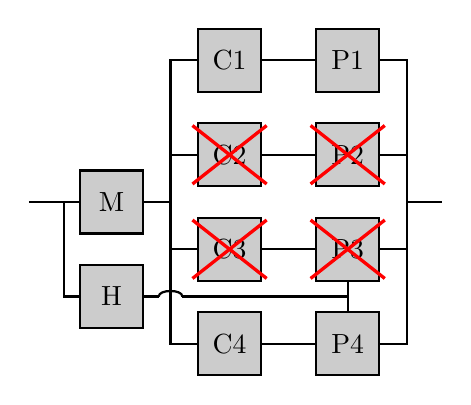
\begin{tikzpicture}
[typeM/.style={rectangle,draw,fill=black!20,thick,inner sep=0pt,minimum size=8mm}, %font=\footnotesize},
 typeC/.style={rectangle,draw,fill=black!20,thick,inner sep=0pt,minimum size=8mm}, %font=\footnotesize},
 typeP/.style={rectangle,draw,fill=black!20,thick,inner sep=0pt,minimum size=8mm}, %font=\footnotesize},
 typeH/.style={rectangle,draw,fill=black!20,thick,inner sep=0pt,minimum size=8mm}, %font=\footnotesize},
 type1/.style={rectangle,draw,fill=black!20,very thick,inner sep=0pt,minimum size=8mm},
 type2/.style={rectangle,draw,fill=black!20,very thick,inner sep=0pt,minimum size=8mm},
 type3/.style={rectangle,draw,fill=black!20,very thick,inner sep=0pt,minimum size=8mm},
 cross/.style={cross out,draw=red,very thick,minimum width=9mm, minimum height=7mm},
 hv path/.style={thick, to path={-| (\tikztotarget)}},
 vh path/.style={thick, to path={|- (\tikztotarget)}}]
\begin{scope}[xscale=1.5, yscale=1.2]
\node[typeM] (M)    at ( 0  , 0  ) {M};
\node[typeC] (C1)   at ( 1  , 1.5) {C1};
\node[typeC] (C2)   at ( 1  , 0.5) {C2};
\node[cross]        at ( 1  , 0.5) {};
\node[typeC] (C3)   at ( 1  ,-0.5) {C3};
\node[cross]        at ( 1  ,-0.5) {};
\node[typeC] (C4)   at ( 1  ,-1.5) {C4};
\node[typeP] (P1)   at ( 2  , 1.5) {P1};
\node[typeP] (P2)   at ( 2  , 0.5) {P2};
\node[cross]        at ( 2  , 0.5) {};
\node[typeP] (P3)   at ( 2  ,-0.5) {P3};
\node[cross]        at ( 2  ,-0.5) {};
\node[typeP] (P4)   at ( 2  ,-1.5) {P4};
\node[typeH] (H)    at ( 0  ,-1  ) {H};
\coordinate (start)  at (-0.7, 0);
\coordinate (startC) at ( 0.5, 0);
\coordinate (startH) at (-0.4, 0);
\coordinate (Hhop1)  at ( 0.4,-1);
\coordinate (Hhop2)  at ( 0.6,-1);
\coordinate (endP)   at ( 2.5, 0);
\coordinate (end)    at ( 2.8, 0);
\path (start)     edge[hv path] (M.west)
      (M.east)    edge[hv path] (startC)
      (startC)    edge[vh path] (C1.west)
                  edge[vh path] (C2.west)
                  edge[vh path] (C3.west)
                  edge[vh path] (C4.west)
      (C1.east)   edge[hv path] (P1.west)
      (C2.east)   edge[hv path] (P2.west)
      (C3.east)   edge[hv path] (P3.west)
      (C4.east)   edge[hv path] (P4.west)
      (endP)      edge[vh path] (P1.east)
                  edge[vh path] (P2.east)
                  edge[vh path] (P3.east)
                  edge[vh path] (P4.east)
                  edge[hv path] (end)
      (startH)    edge[vh path] (H.west)
      (H.east)    edge[hv path] (Hhop1)
      (Hhop1)     edge[thick,out=90,in=90] (Hhop2)
      (Hhop2)     edge[hv path] (P3.south)
                  edge[hv path] (P4.north);
\end{scope}
\end{tikzpicture}
\end{document}
